\documentclass[11pt,leqno]{book}
\textwidth 13.5cm
\textheight 18.5cm
\topmargin 0in
\parindent 0.5cm
\oddsidemargin 0.5in
\evensidemargin 0.5in
\usepackage{amssymb}
\usepackage{amsmath}
\usepackage{graphicx,wrapfig,url,rotating,array}
\usepackage{fan}
\usepackage{subcaption}
\usepackage{placeins}
%
\def\bibname{{\Large\bf References}}
\def\thebibliography#1{\addvspace{3em}\noindent
\noindent \bibname  \list
 {[\arabic{enumi}]}{\settowidth\labelwidth{[#1]}\leftmargin\labelwidth
 \advance\leftmargin\labelsep
 \usecounter{enumi}}
 \def\newblock{\hskip .11em plus .33em minus .07em}
 \sloppy\clubpenalty4000\widowpenalty4000
 \sfcode`\.=1000\relax}
\let\endthebibliography=\endlist
%
\usepackage[english]{babel}
%
\pagestyle{fancy}
\footrulewidth 0pt
\headrulewidth 0.5pt
\lfoot[\thepage]{} \cfoot[]{} \rfoot[]{\thepage}
\lhead[Geometric Visualization of a Polygon Area Partitioning]{ESGI'132} \chead[]{} \rhead[ESGI'132]{Geometric Visualization of a Polygon Area Partitioning}
%
\def\efig#1#2{\includegraphics[width=#2mm]{#1}}
\def\efigsc#1#2{\includegraphics[scale=#2]{#1}}
\def\TTT{\end{document}}
\def\bt{\begin{tabular}}
\def\et{\end{tabular}}
\def\cl{\centerline}
\def\mc{\multicolumn}
%
\def\diag{\mathop{\rm diag}}
\thispagestyle{empty}
\newcommand{\sect}[1]{\vskip7mm\par{\large \bf #1}}
\newcommand{\subsect}[1]{\vskip 3mm\par{\bf#1}}
%
 \def\hlst{\setlength{\topsep}{1pt}\setlength{\partopsep}{1pt}%
 \setlength{\parsep}{1pt}\setlength{\itemsep}{\parskip}}
%
\begin{document}
%
\begin{center}
\textbf{\LARGE Geometric Visualization of a Polygon Area Partitioning}

\vspace*{5mm}
%
Todor Balabanov,
Stanislav Darachev,
Ivan Jordanov,
Aleksandar Karakushev,
Nikolai Kitanov,
Alexander Manov,
Georgi Nikolov,
Spasimir Nonev,
Zdravka Nedyalkova,
Emiliyan Rogachev,
Natasha Stojkovikj,
Petar Tomov,
Iliyan Zankinski
%
\end{center}
%
\date{18-22 Sep 2017}
%
\sect{Abstract}
%
In the process of modeling sewerage networks, the main component is the drained area (catchment) from which water is collected to each conduit (pipe). If the area for a single subcatchment is derived from a mathematical model, we have to create the geometry of that territory. For visualization purpose, we need to find geometric partitioning of the polygon.

In this paper we propose 6 solutions for geometric visualization of a polygon area partitioning.

\textit{Key words}: visualization, polygon area partitioning, optimal cutting problem

\sect{1.~Introduction}

In the process of modeling sewerage networks, the main component is the drained area (catchment) from which water is collected to each conduit (pipe). If the area for a single sub-catchment is derived from a mathematical model, we have to create the geometry of that territory, Exactly, in this paper, we want to make geometric visualization for partitioning of a given living area, with respect to the known water debit, relative to each pipe. If each pipe is represent as edges and these edges formed polygon  then our main goal is to make geometric visualization of a polygon area partitioning.  

Despite, this problem is important in hydrology, there is little published information in the hydrological literature. 

In the paper \cite{han:bra:1}, two approaches for automated generation of  Thiessen polygons are considered. Exactly, triangulation method and grid method are described and the ways for their implementation in hydrological applications is given. Also, procedure to derive the relationship between the catchment area, grid size, and accuracy indicator based on weighted mean error is described. 

In the paper \cite{mai:mik:1}, web-based urban water management modeling platform for simplifying the setup and use of complex integrated models is presented.  The paper demonstrates how flooding behavior of new urban developments can easily be assessed with the web platform, i.e. to inform discussions in interdisciplinary and interactive stakeholder workshops.  Also, in the paper the workflow of the used DynaMind model is shown. The inputs are the user defined catchment are are presented as polygons and an existing or user defined combined sewer system model which will be affected by the new catchments. This polygon is divided into several smaller polygons/sub- catchments by normal distributing new inlet nodes within the polygon and creating a Voronoi diagram on the bases of these nodes. 

Paper \cite{lay:day:1} is focused on the generation of three dimensional models of large urban/suburban environments. Automated tools can be used to provide a rapid coarse model of a city. These techniques can be tailored to generate geometry of appropriate complexity for real-time rendering, thereby negating the need for the simplification stage. In the paper, roof modelling for rectilinear polygons is used, and it is described  procedure to partition  on polygon into rectangles.

Paper \cite{lockie:1} outlines the technical capability and functionality of SWMM. Also the advantages, disadvantage and applicability of SWMM are discussed and a brief comparison between SWMM and other common hydraulic models is presented. The hydraulic engine of SWMM has been proven and tested more than 40 years and is reported the most widely applied stormwater model in US and New Zealand.

\begin{figure}[h!]
\centering
\begin{subfigure}{.5\textwidth}
  \centering
  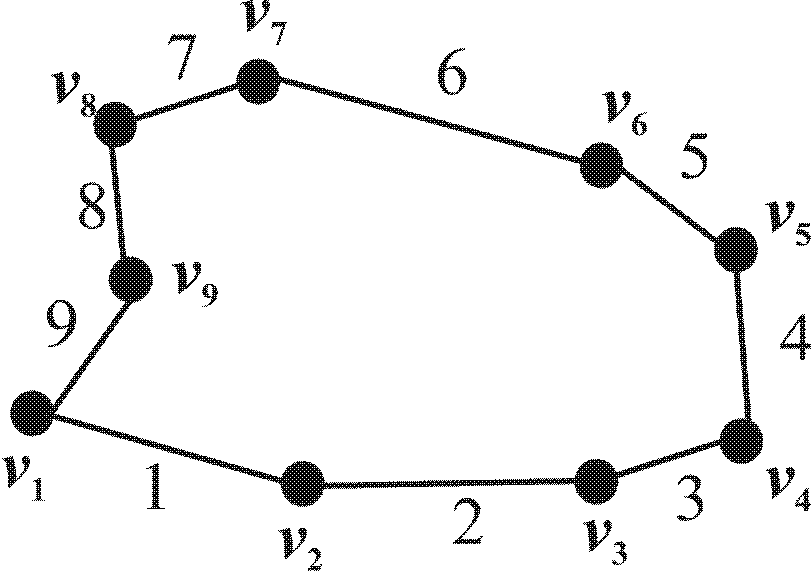
\includegraphics[width=.5\linewidth]{pic01.png}
  \caption{Input polygon.}
  \label{fig:sub1}
\end{subfigure}%
\begin{subfigure}{.5\textwidth}
  \centering
  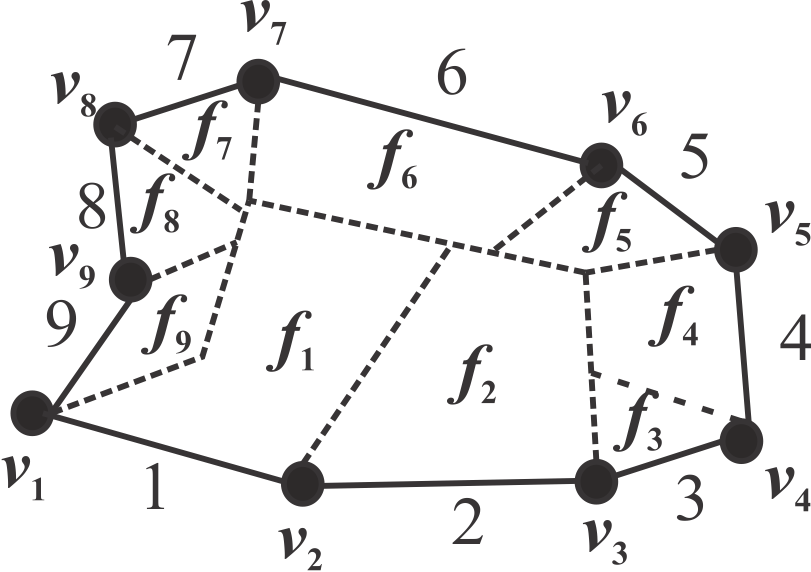
\includegraphics[width=.5\linewidth]{pic03.png}
  \caption{Possible solution.}
  \label{fig:sub2}
\end{subfigure}
\caption{Problem input/output representation.}
\label{fig:one}
\end{figure}
\FloatBarrier

Digital elevation model (DEM) can be used to automatically generate catchment areas. San Francisco Department of Public Work (SF DPW) applied similar techniques at a fine resolution.  These results are used to study pipe hydraulics for San Francisco’s several systems. To automated the drainage catchment delineation process,  computer script in ArcGIS Model Builder called the Urbane Drainage Model is created. The Urbane Drainage Model is based on the commonly used “sleepiest path” approach,  using a gridded evaluation model, catchment areas were delineated for the City of San Francisco. A sub-catchment was created for each drain in the area.

The problem  mathematically is formulated in the following way:

A polygon $P$ (corresponding to the catchment) is given with the Cartesian coordinates of its vertices (corresponding to Manholes) and its edges $i= 1, \ldots, N$, (corresponding to pipes). Thus, the area of the polygon $F$ is also known. With each edge, we associate a relative area $f_i$ (corresponding to the relative water debit in percentages), where  $100\% = \sum f_i$.

The vertices of the polygon are denoted with $v_i$, $ i = 1, \ldots, N$.
For visualization purposes, we look for a geometric partitioning of the polygon, such that the area of the$i$-th part is equal to $f_i$.

For the given data in Fig. \ref{fig:sub3}.

\begin{figure}[h!]
\centering
\begin{subfigure}{.5\textwidth}
  \centering
  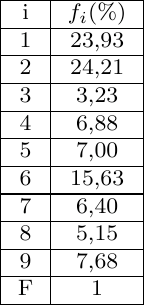
\includegraphics[width=.4\linewidth]{pic07.png}
  \caption{Table data.}
  \label{fig:sub3}
\end{subfigure}%
\begin{subfigure}{.5\textwidth}
  \centering
  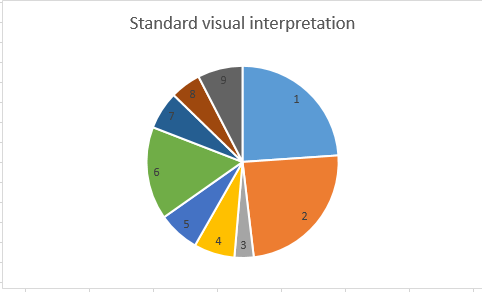
\includegraphics[width=.8\linewidth]{pic02.png}
  \caption{Pie chart.}
  \label{fig:sub4}
\end{subfigure}
\caption{Test case data.}
\label{fig:two}
\end{figure}
\FloatBarrier

Standard visual interpretation is given Fig. \ref{fig:sub4}.

We looking for the following visual (geometrical) interpretation (Fig. \ref{fig:sub2})

\sect{2.~Solution approaches}

\subsect{2.1.~Monte Carlo Flooding}

With this algorithm the polygon will be divided in $N$ irregular shapes. Let the area of the figures is noticed by $c_i, i = 1. \ldots, N$.  Following is the pseudocode of the proposed MCFA.

\noindent\rule{\textwidth}{1pt}
\begin{itemize}
\item[Step 1.]  For all edges, find middle point of the edge, $t_i(x,y)$.
\item[Step 2.]  For all points $t_i(x,y), i=1,\ldots, N$, form figures $IF_i$ from the nearest points on the point $t_i(x,y)$. 
\item[Step 3.] Find areas of the formed figures, $c_i, i = 1, \ldots, N$.
\item[Step 4.] For $i = 1$ to $N$
\begin{itemize}
  \item[Step 4.1]  While ($c_i \leq f_i$)
  \item[Step 4.2]  Add nearest points to boundary on figure $IF_i$ in the figure $IF_i$. 
\end{itemize}
\end{itemize}
\noindent\rule{\textwidth}{1pt}

The final result of the algorithm is similar to liquid foolding from different sides.

\subsect{2.2.~Genetic Algorithm}

First, we choose $N$ point, $b_i$  on random way, where $N$ is a number of edges.

Each of these points, with the end points from the edges of the polygon will be connected, and on this ways we form $N$ triangles  $T_i$. The area of the triagles $T_i, i=1, \ldots, N $ will be denoted with $a_i$. The area of the polygon, outside of the triangles is denoted with $W$.  This is shown on Fig. \ref{fig:sub6}.

We form following sums:
$$B= count( b_i), i =1, \ldots, N$$
$$ W= count(w_{(x,y)})$$ where $w_{ (x,y)}\notin T_i, \forall{ T_i}, i=1, \dots, N$
$$ A= \sum_{(a_i - f_i)>0}(a_i-f_i)$$
Now, we regard one triangle.  Let, for the random point $t(x_i, y_i) \in T_i$,  $d_{ij}$  is distance from the point to the $i$-edge from the polygon. 

\begin{figure}[h!]
\centering
\begin{subfigure}{.5\textwidth}
  \centering
  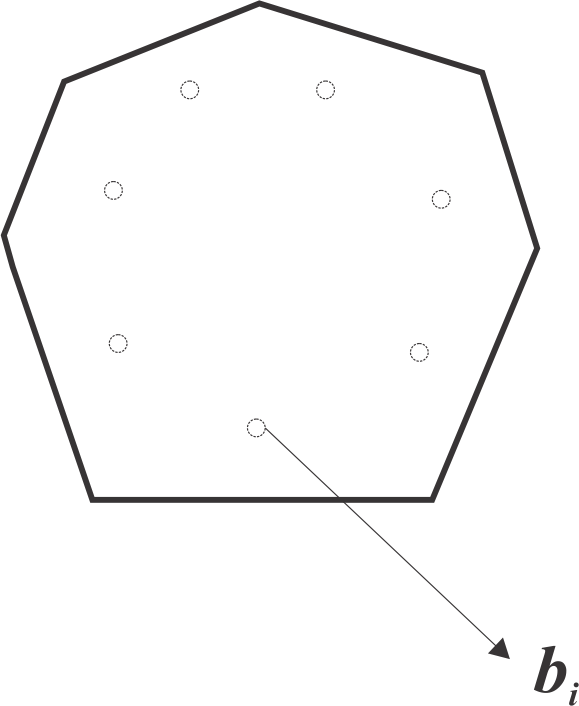
\includegraphics[width=.5\linewidth]{pic04.png}
  \caption{Point selection near to each side.}
  \label{fig:sub5}
\end{subfigure}%
\begin{subfigure}{.5\textwidth}
  \centering
  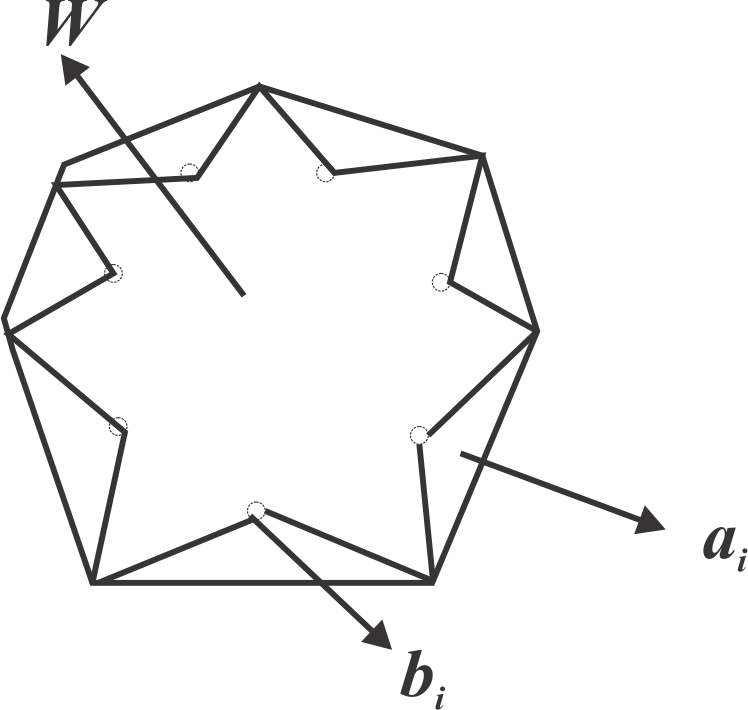
\includegraphics[width=.6\linewidth]{pic05.png}
  \caption{Form initial triangles to each side.}
  \label{fig:sub6}
\end{subfigure}
\caption{Selection of initial sub-polygons related to each side of the polygon.}
\label{fig:three}
\end{figure}

The  following sums are formed: $$d_i = \frac{\sum_{j=1}^k d_{ij}}k$$
where $k$ is a  total number of the point on the triangle  and

$$D = \sum_{i=1}^N d_i$$.

We need to estimated cost function
$$cost f = D+W + A + B$$.

\begin{figure}[h!]
  \centering
  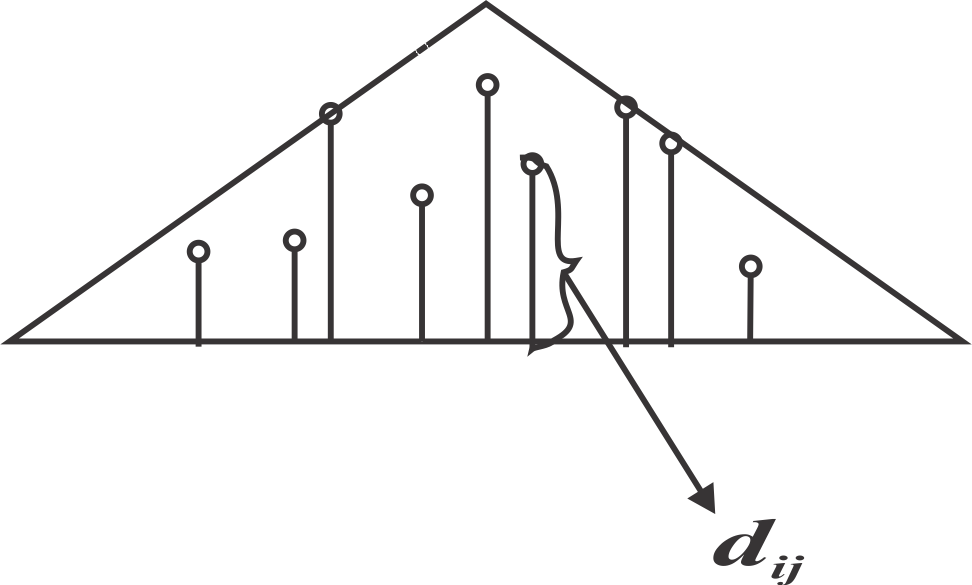
\includegraphics[width=.5\linewidth]{pic06.png}
  \caption{Calculate average distance of all pixels in the sub-plygon to the polygon side.}
\label{fig:four}
\end{figure}
\FloatBarrier

Our goal is to minimized the cost function. Since, we need to minimize $D, W, A, B$. The set of values for $W$ is $[0, count( p(x_i, y_i))], \forall p(x_i, y_i) \in P$. From , this we can conclude, that optimal value for W is 0.
The set of values for $A$ is $[0, count (p(x_i, y_i))], \forall p(x_i, y_i) \in P$, we conclude that minimal value of $A$ is 0. And, the $B$ have set of values $[N,count( p(x_i, y_i))], \forall p(x_i, y_i) \in P$, and minimal value from $B$ is $N$, where $N$ is a number of edges of the polygon.
if we succeed to minimize $A, B, W$, we will give the minimum value of the cost function.

\subsect{2.3.~Percent Distributed Clustering}

The given area is divided into a fine grid of pixels. The sides of the polygon are also divided into sixty line segments each. For each pixel of the area the algorithm finds the line segment that gives the lowest value for the distance between the pixel and the line segment multiplied by 100 minus the required percentage of the area: distance * (100 - f(x)). The side that the line segment belongs to is the side that the area taken by the pixel will drain into.

\subsect{2.4.~Offsetting Polygon}

The main idea of the offsetting polygon approach is to fill the initial polygon with smaller ones of which each side is parallel to the corresponding one of the initial polygon. The initial algorithm is the following:

\noindent\rule{\textwidth}{1pt}
\begin{itemize}

\item[Step 1.] Draw a parallel segment to each side of the polygon, creating a smaller polygon inside each with an offesetting distance $h$. 
\item[Step 2.] Connect each of the corresponding vertices of each polygon and calculate the area of the trapezoids created.
\item[Step 3.] Calculate the area of the created trapezoids and check if it fits the data.
\begin{itemize}
\item[Step 3.1] If the area doesn't fit we continue with creating parallel polygons.
\item[Step 3.2] If the desired area is accomplished, fix the side of the corresponding trapezoid and stop drawing parallel sides for it.
\end{itemize}
  \item[Step 4] Continue \textit{Step 2} until the data is fitted.
\end{itemize}
\noindent\rule{\textwidth}{1pt}

The initial algorithm applied worked very well for convex polygons. But when the algorithm was tested on a concave polygon the results were unsatisfying and this approach needed to be modified. The modifications were in the form of defining a different offsetting step $h$ for each side i.e. we will have $n$ different distances, where $n$ is the number of the polygon's sides. Following this approach, we end up with the concave angle's corresponding sides intersect with the opposite side. At this iteration of the algorithm, we modify the distance between the parallel sides so that they cross the opposite side at one point. As a result, we obtain two smaller polygons for which we apply the same algorithm. By the end with this modified approach we get a triangle(s) which area to side distributions can be found easily.

\sect{3.~Experimens and Results}

\subsect{3.1.~Monte Carlo Flooding}

Monte Carlo Flooding is very efficient heuristics it it has few disadvantages in the solution of the problem. The biggest disadvantage is related with the fact that 2D space is divided in shapes similar to semi-circles when polygons are required. Second biggest disadvantage is about optimal distribution of the sub-areas, which is clearly visible in Fig. \ref{fig:sub7}. 

\begin{figure}[h!]
\centering
\begin{subfigure}{.5\textwidth}
  \centering
  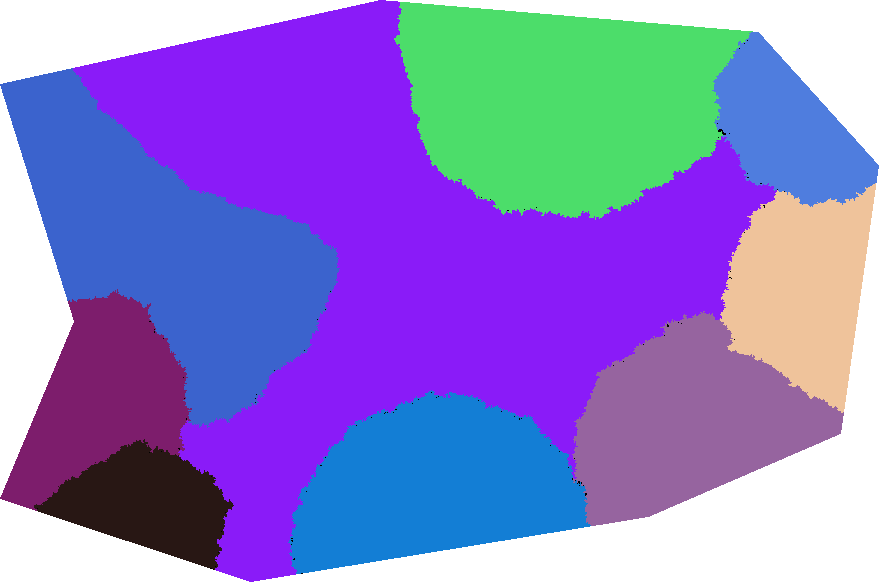
\includegraphics[width=.5\linewidth]{pic08.png}
  \caption{Test case 1.}
  \label{fig:sub7}
\end{subfigure}%
\begin{subfigure}{.5\textwidth}
  \centering
  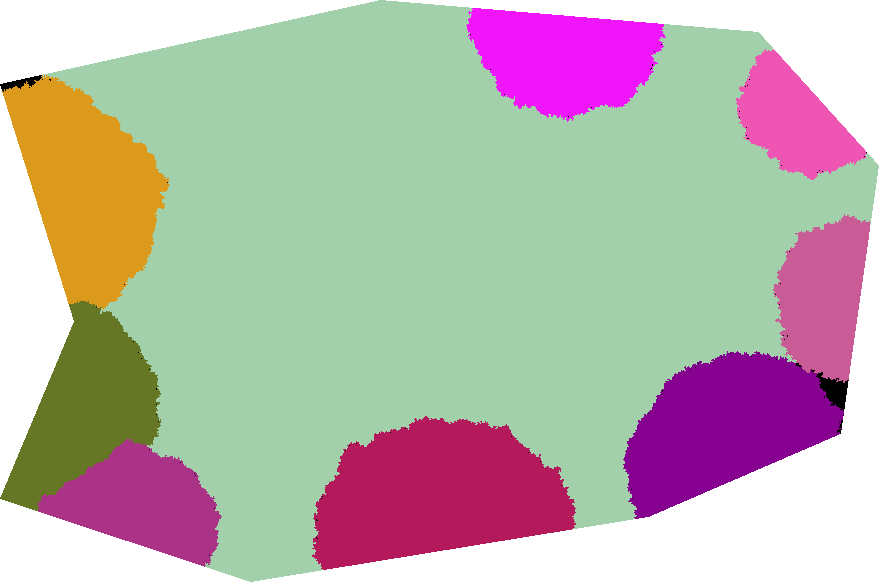
\includegraphics[width=.5\linewidth]{pic09.png}
  \caption{Test case 2.}
  \label{fig:sub8}
\end{subfigure}
\caption{Monte Carlo Flooding algorithm results.}
\label{fig:five}
\end{figure}
\FloatBarrier

\subsect{3.2.~Percent Distributed Clustering}

Percent Distributed Clustering divides the polygon in straight lines.

\begin{figure}[h!]
\centering
\begin{subfigure}{.5\textwidth}
  \centering
  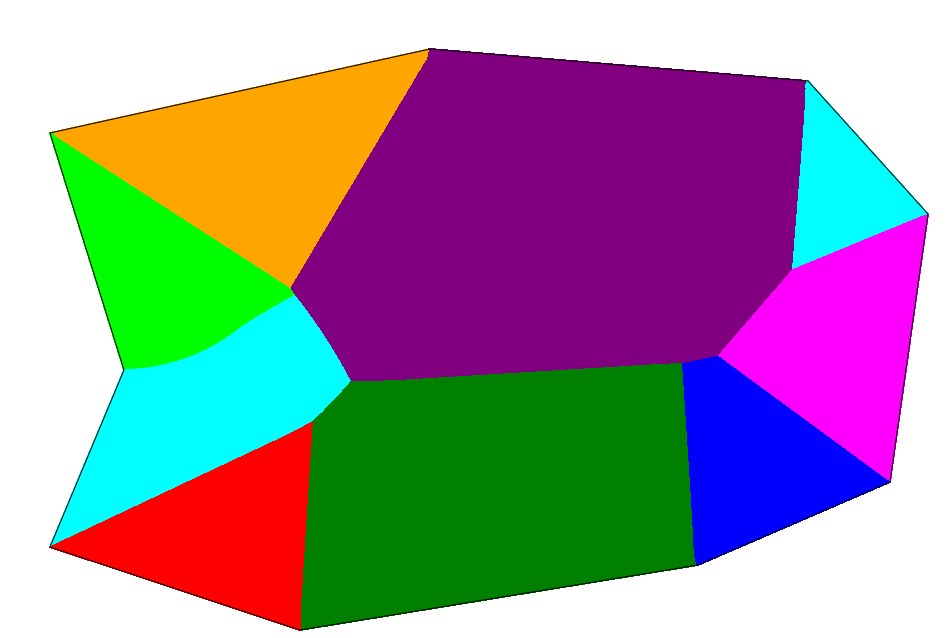
\includegraphics[width=.5\linewidth]{pic10.png}
  \caption{Test case 1.}
  \label{fig:sub9}
\end{subfigure}%
\begin{subfigure}{.5\textwidth}
  \centering
  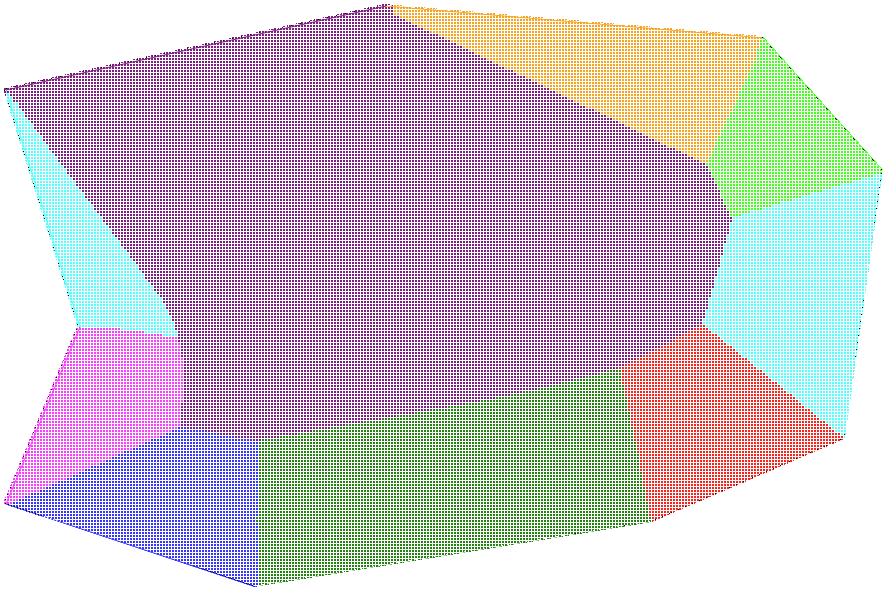
\includegraphics[width=.5\linewidth]{pic11.png}
  \caption{Test case 2.}
  \label{fig:sub10}
\end{subfigure}
\caption{Percent Distributed Clustering algorithm results.}
\label{fig:six}
\end{figure}
\FloatBarrier

\subsect{3.3.~Offsetting Polygon}

Offsetting polygon method divides the polygon into smaller polygons with sides parallel to the initial one. Figure \ref{fig:sub11} shows the intitial step of the algorithm. Figure \ref{fig:sub12} is the result from the unmodified algorithm, ran on a concave polygon. Figure \ref{fig:sub13} contains the step with the intersecting parts of the polygon and a final result of two smaller triangles.

\begin{figure}[h!] 
\centering
\begin{subfigure}{.5\textwidth}
  \centering
  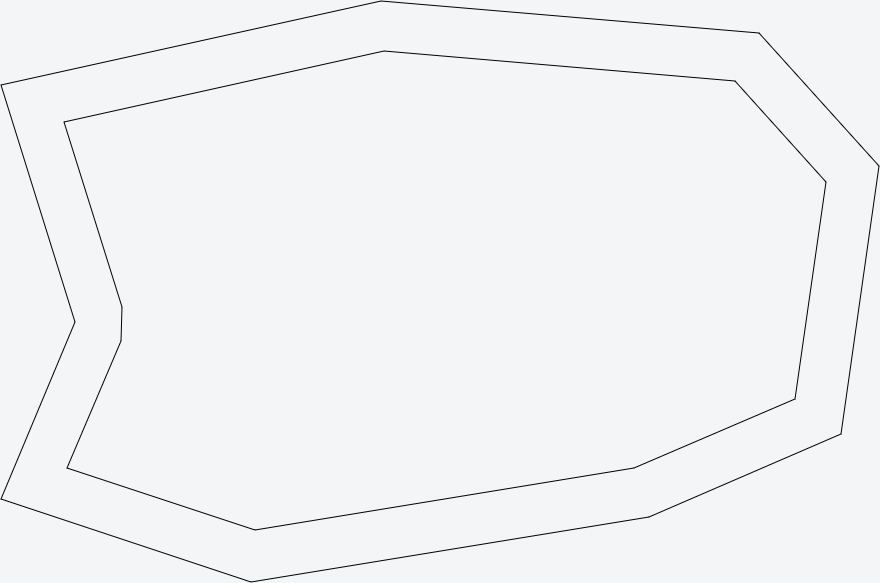
\includegraphics[width=.5\linewidth]{pic12.png}
  \caption{Initial step.}
  \label{fig:sub11}
\end{subfigure}%
\begin{subfigure}{.5\textwidth}
  \centering
  
\includegraphics[width=.5\linewidth]{pic13.png}
  \caption{Final result.}
  \label{fig:sub12}
\end{subfigure}
\caption{Offsetting Polygon algorithm results.}
\label{fig:seven}
\end{figure}
\FloatBarrier

Figure 8 shows the interception step of the modified algorithm and Figure 9 shows the final result of the algorithm.

\begin{figure}[h!]
  \centering
  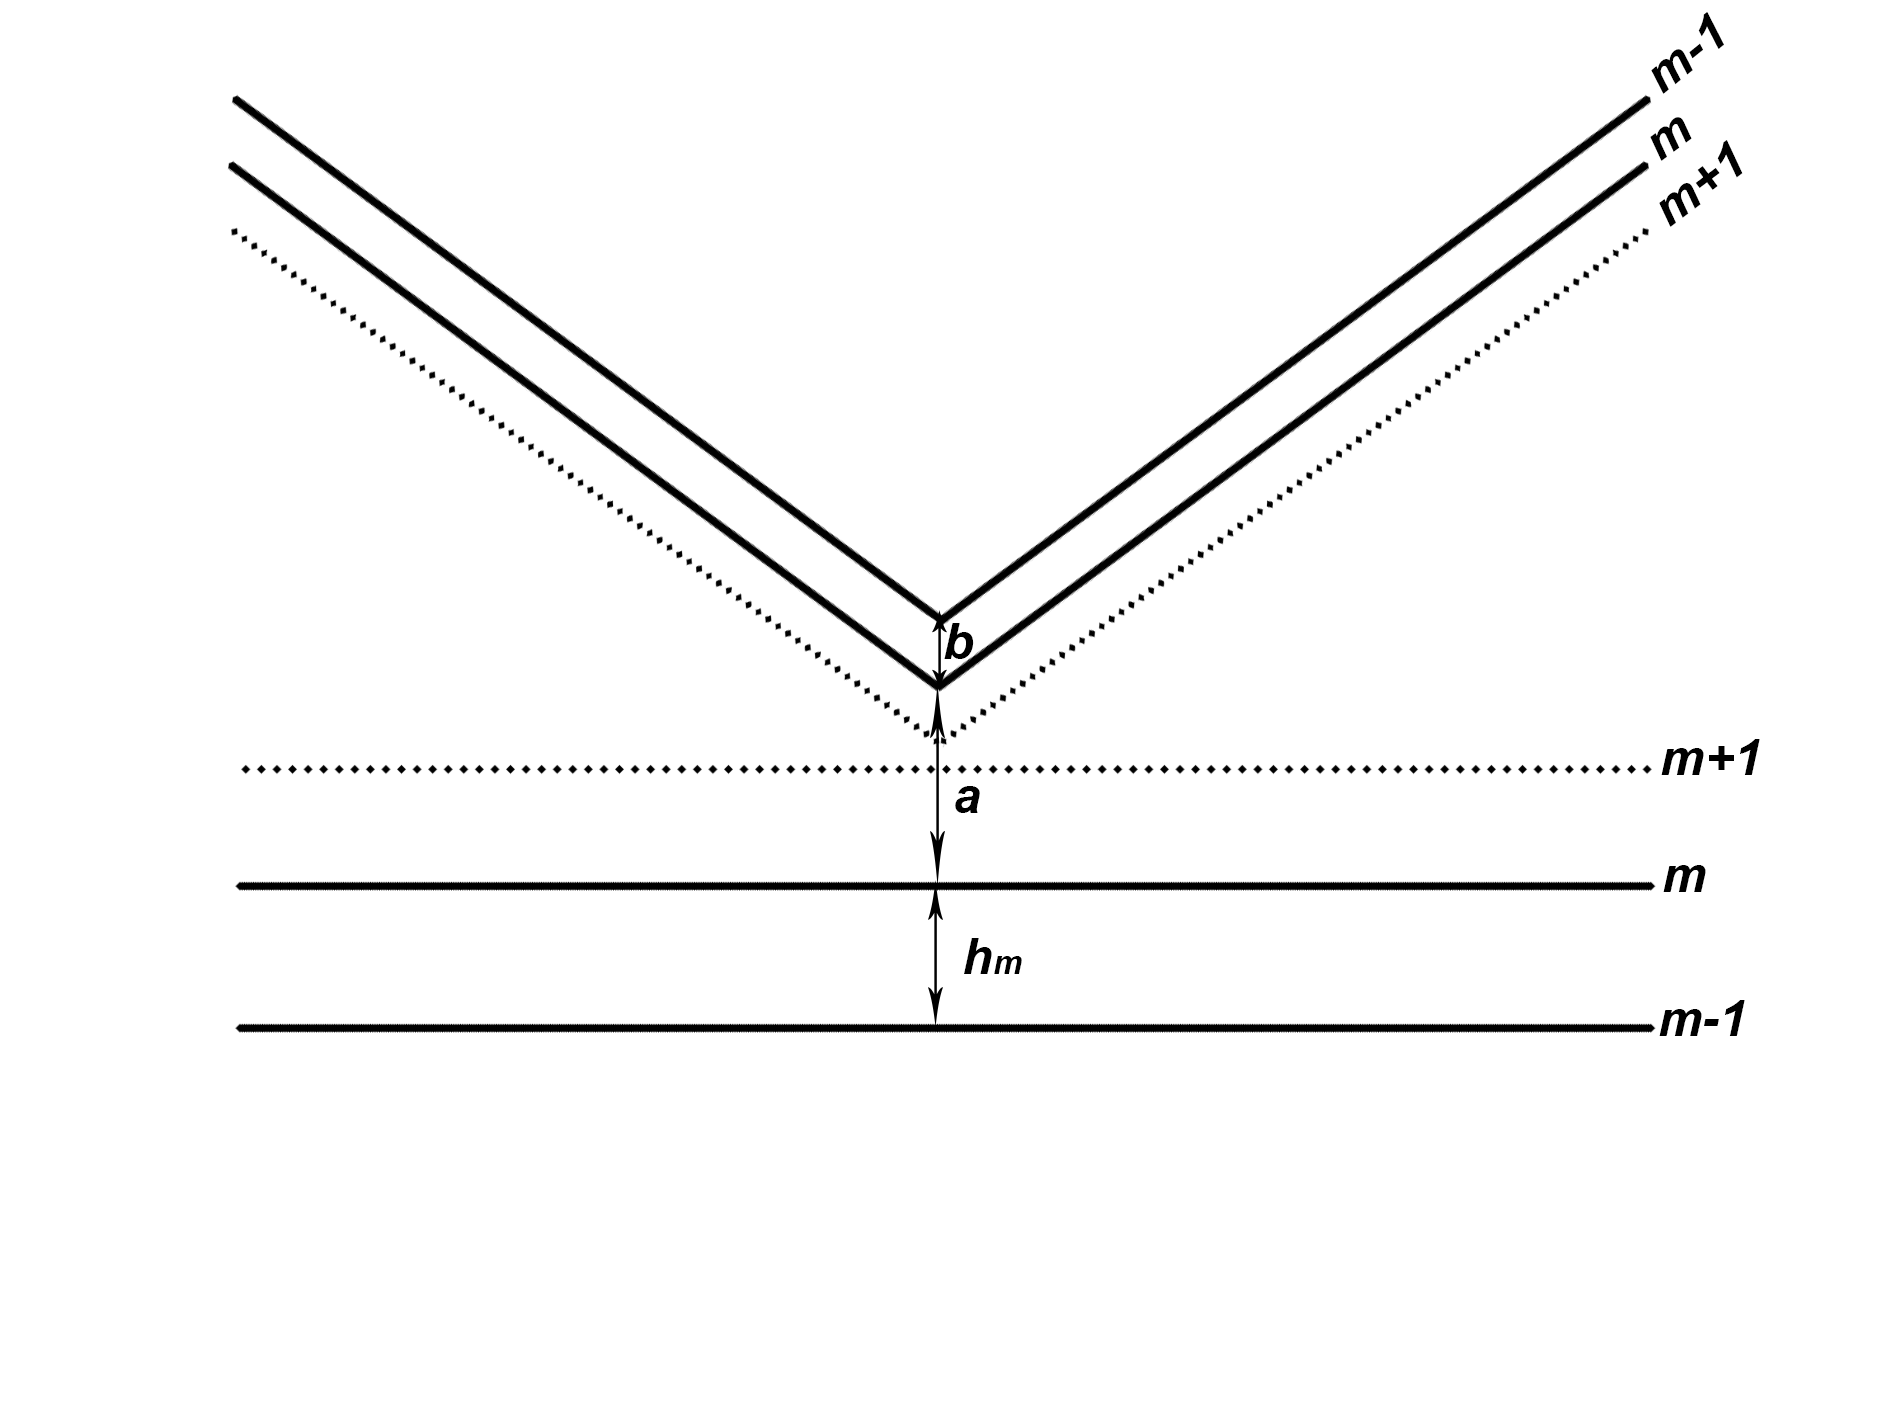
\includegraphics[width=.6\linewidth]{pic15.png}
  \caption{Intercepting part of the algorithm.}
\end{figure}
\FloatBarrier

\begin{figure}[h!]
  \centering
  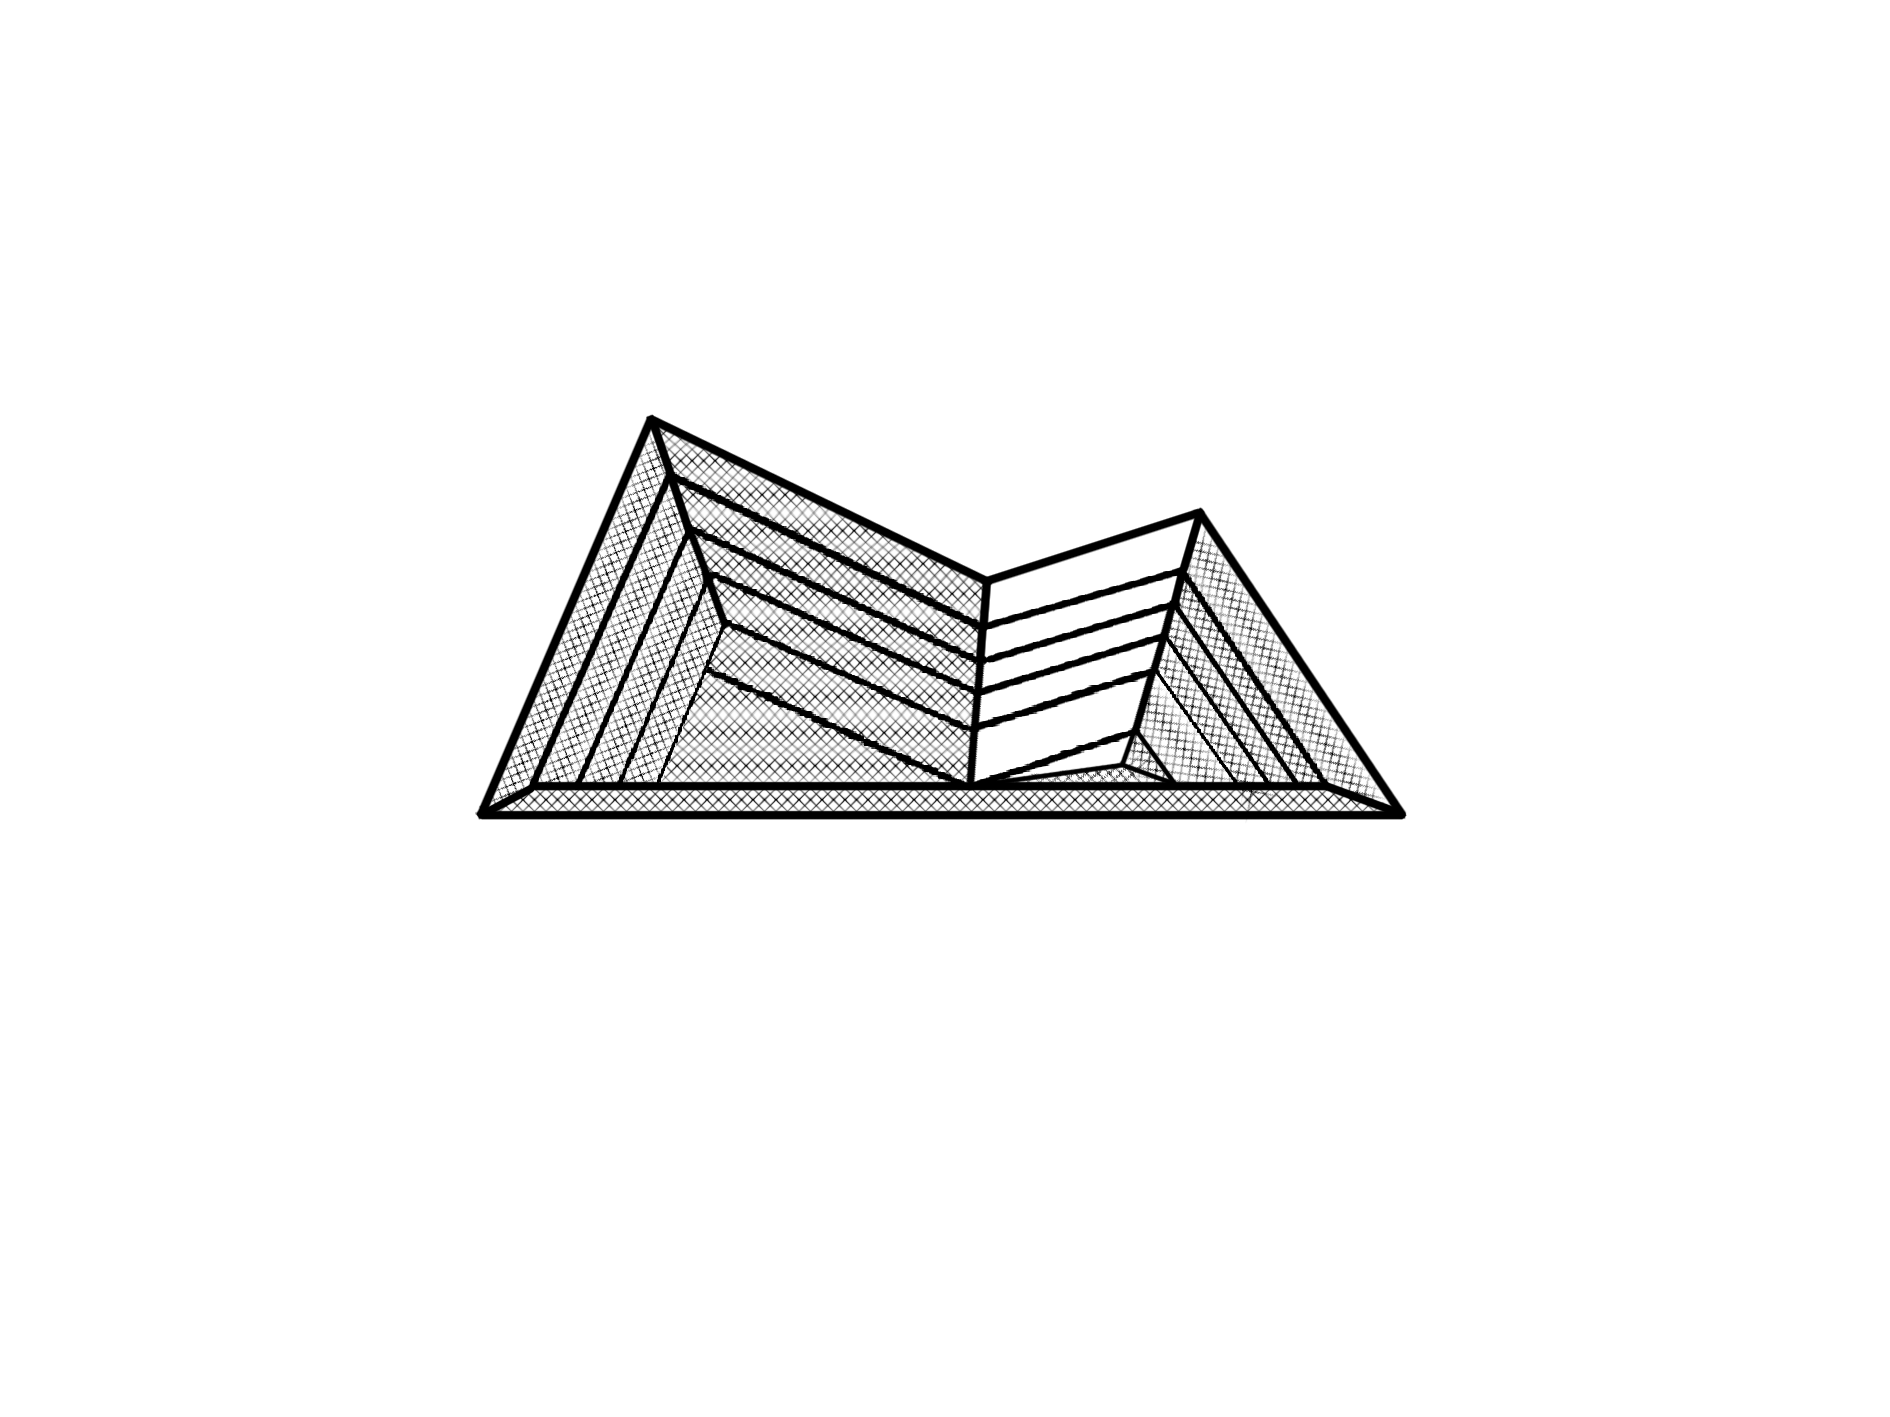
\includegraphics[width=.9\linewidth]{pic14.png}
  \caption{Modified offsetting polygon algorithm.}
\end{figure}
\FloatBarrier

\sect{Conclusions}

Experimental results show that usage of Percent Distributed Clustering and Offsetting Polygon can produce much better accepted results than Monte Carlo Flooding.

\sect{Acknowledgements}

Faculty of Mathematics and Informatics, Sofia University St. Kliment Ohridski, Institute of Information and Communication Technologies, Bulgarian Academy of Sciences, Institute of Mathematics and Informatics, Bulgarian Academy of Sciences, European Consortium for Mathematics in Industry, Skyscanner Ltd., Vodostroitelno Predpriatie Ltd., Academy of Music, Dance and Fine Arts - Plovdiv

\def\bibname{{\Large\bf References}}
\begin{thebibliography}{99}
%
\bibitem{han:bra:1} Han, D., and Bray, M. “Automated Thiessen polygon generation”, Water resources research, vol. 42, 2006.
%
\bibitem{mai:mik:1} Mair M., Mikovits C., Sengthaler M., Schoepf M., Kinzel H., Urich C., Kleidorfer M., Sitzenfrei R. and Rauch W, “The application of a Web-geographic information system for improving urban water cycle modelling “  Water Science and Technology 70(11), 2014, pp.1838-1846.
%
\bibitem{lay:day:1} Laycock R. G., Day A. M.”Automatically generating large urban environments based on the footprint data of buildings”, Proceedings of the eighth ACM symposium on Solid modeling and applications (New York, NY, USA), ACM Press, 2003, pp. 346–351.
%
\bibitem{lockie:1} Lockie T, “Catchment Modelling using SWMM” Modelling Stream at the 49th Water New Zealand Annual Conference and Expo, 2009.
%
\end{thebibliography}
%
\end{document}
